%% 2/18/2016
%%%%%%%%%%%%%%%%%%%%%%%%%%%%%%%%%%%%%%%%%%%%%%%%%%%%%%%%%%%%%%%%%%%%%%%%%%%%
% AGUJournalSample.tex: this sample file is for articles formatted with LaTeX
%
% This sample file includes commands and instructions
% given in the order necessary to produce a final output that will
% satisfy AGU requirements.
%
% PLEASE DO NOT USE YOUR OWN MACROS
% DO NOT USE \newcommand, \renewcommand, or \def.
%
% FOR FIGURES, DO NOT USE \psfrag or \subfigure.
% DO NOT USE \psfrag or \subfigure commands.
%
%%%%%%%%%%%%%%%%%%%%%%%%%%%%%%%%%%%%%%%%%%%%%%%%%%%%%%%%%%%%%%%%%%%%%%%%%%%%
%
% All questions should be e-mailed to latex@agu.org.
%
%%%%%%%%%%%%%%%%%%%%%%%%%%%%%%%%%%%%%%%%%%%%%%%%%%%%%%%%%%%%%%%%%%%%%%%%%%%%
%
% Step 1: Set the \documentclass
%
% There are two options for article format:
%
% 1) PLEASE USE THE DRAFT OPTION TO SUBMIT YOUR PAPERS.
% The draft option produces double spaced output.
% 
% 2) numberline will give you line numbers.

% Tip:
%  To add line numbers to lines in equations:
%  \begin{linenomath*}
%  \begin{equation}
%  \end{equation}
%  \end{linenomath*}

%% To submit your paper:
\documentclass[linenumbers,draft]{agujournal}

% Now, type in the journal name: \journalname{<Journal Name>}
% ie,
\journalname{Earth and Space Science}

%% Choose from this list of Journals:
%
% JGR-Atmospheres
% JGR-Biogeosciences
% JGR-Earth Surface
% JGR-Oceans
% JGR-Planets
% JGR-Solid Earth
% JGR-Space Physics
% Global Biochemical Cycles
% Geophysical Research Letters
% Paleoceanography
% Radio Science
% Reviews of Geophysics
% Tectonics
% Space Weather
% Water Resource Research
% Geochemistry, Geophysics, Geosystems
% Journal of Advances in Modeling Earth Systems (JAMES)
% Earth's Future
% Earth and Space Science


%% ------------------------------------------------------------------------ %%
%
%  ENTER Title Page commands:
%
%% ------------------------------------------------------------------------ %%

% (A title should be specific, informative, and brief. Use
% abbreviations only if they are defined in the abstract. Titles that
% start with general terms then specific results are optimized in
% searches)

% Example: \title{This is a test title}

% (List authors by first name or initial followed by last name and
% separated by commas. Use \affil{} to number affiliations, and
% \thanks{} for author notes.  
% Additional author notes should be indicated with \thanks{} (for
% example, for current addresses). 

% Example: \authors{A. B. Author\affil{1}\thanks{Current address, Antartica}, B. C. Author\affil{2,3}, and D. E.
% Author\affil{3,4}\thanks{Also funded by Monsanto.}}

% (include name and email addresses of the corresponding author.  More
% than one corresponding author is allowed in this LaTeX file and for
% publication; but only one corresponding author is allowed in our
% editorial system.)  

%% Corresponding Author:
% Corresponding author mailing address and e-mail address:

% Example: \correspondingauthor{First and Last Name}{email@address.edu}

% Authors are individuals who have significantly contributed to the
% research and preparation of the article. Group authors are allowed, if
% each author in the group is separately identified in an appendix.)

% \affiliation{1}{First Affiliation}
% \affiliation{2}{Second Affiliation}
% \affiliation{3}{Third Affiliation}
% \affiliation{4}{Fourth Affiliation}

%% Keypoints, final entry on title page.
% Example: 
% \begin{keypoints}
% \item	List up to three key points (at least one is required)
% \item	Key Points summarize the main points and conclusions of the article
% \item	Each must be 100 characters or less with no special
% characters or punctuation 
% \end{keypoints}

%% \begin{abstract} begins second page 

%%%%%%%%%%%%%%%%%%%%%%%%%%%%%%%%%%%%%%%%%%%%%%%%%%%%%%%%%%%%%%%%%%%%%
% Track Changes:
% To add words, \added{<word added>}
% To delete words, \deleted{<word deleted>}
% To replace words, \replace{<word to be replaced>}{<replacement word>}
% To explain why change was made: \explain{<explanation>}

% At the end of the document, use \listofchanges, which will list the
% changes and the page and line number where the change was made.

% When final version, \listofchanges will not produce anything,
% \added{} word will be printed, \deleted{} will take away the word,
% \replaced{}{} will print only the 2nd argument.
% \explain will not print anything.

% Optional argument:
% You can also add additional information to be printed with the list
% of changes, to indicate the initials of the person changing the text,
% and the time and/or date of the change, or any other comment by using
% the optional [] argument:
% \added[AH, 3:30pm, Feb 18, 2016]{added term}
% will yield 
% [AH, 3:30pm, Feb 18, 2016] added term on page...
%%%%%%%%%%%%%%%%%%%%%%%%%%%%%%%%%%%%%%%%%%%%%%%%%%%%%%%%%%%%%%%%%%%%%

\begin{document}

%% ------------------------------------------------------------------------ %%
%
%  TITLE
%
%% ------------------------------------------------------------------------ %%


\title{FITS format for planetary surfaces: definitions, applications and best practices.}


%% ------------------------------------------------------------------------ %%
%
%  AUTHORS AND AFFILIATIONS
%
%% ------------------------------------------------------------------------ %%

 \authors{C. Marmo\affil{1},
 T. M. Hare\affil{2},
 S. Erard\affil{3},
 B. Cecconi\affil{3},
 M. Minin\affil{4},
 A. P. Rossi\affil{4} ...}

\affiliation{1}{GEOPS, Univ. Paris-Sud, CNRS, Univ. Paris-Saclay, Orsay, France}
\affiliation{2}{U. S. Geological Survey, Astrogeology Science Center, Flagstaff, AZ, USA}
\affiliation{3}{LESIA, Observatoire de Paris, PSL Research University, CNRS, Sorbonne Universités, UPMC Univ. Paris 06, Univ. Paris Diderot, Sorbonne Paris Cité, Meudon, France}
\affiliation{4}{Jacobs University, Bremen, Germany}
%\affiliation{5}{}


%% Corresponding Author
%(include name and email addresses of the corresponding author.  More
%than one corresponding author is allowed in this Word file and for
%publication; but only one corresponding author is allowed in our
%editorial system.)  

\correspondingauthor{C. Marmo}{chiara.marmo@u-psud.fr}

%  List up to three key points (at least one is required)
%  Key Points summarize the main points and conclusions of the article
%  Each must be 100 characters or less with no special characters or punctuation 

\begin{keypoints}
\item Inter-operable data formats 
\item Planetary data standards
\item Data processing and visualization
\end{keypoints}

%% ------------------------------------------------------------------------ %%
%
%  ABSTRACT
%
%% ------------------------------------------------------------------------ %%


\begin{abstract}
Planetary science is a vast field of investigation that brings together several
research communities (geologists, astronomers, physicists, geochemists, etc.),
and produces an impressively growing amount of heterogeneous data.
Planetary surface research continues to evolve from mostly visual assessment
to more automated quantitative analysis.
Interoperability and openness of data formats and processing techniques are
becoming a necessity, to avoid the risk of being unable to efficiently extract
scientific information from the data, and to guarantee the reproducibility of
the scientific results.
This paper will describe how Flexible Image Transport System (FITS) can be used
in planetary surface investigations, and how its metadata can easily be inserted
in the PDS 4 metadata distribution model.
FITS format is open and flexible, largely implemented in open and efficient
processing tools.
Those reasons make FITS format appropriate for large amounts of raster data
processing.
The purpose of this approach is to make easier data mining and re-processing in
Planetary Surface investigations, promoting general software based on those
standards.
More than capturing a formal data model, FITS description for those data aims to
simplify operational logistics.
\end{abstract}

%% ------------------------------------------------------------------------ %%
%
%  TEXT
%
%% ------------------------------------------------------------------------ %%

%%% Suggested section heads:
% \section{Introduction}
% 
% The main text should start with an introduction. Except for short
% manuscripts (such as comments and replies), the text should be divided
% into sections, each with its own heading. 

% Headings should be sentence fragments and do not begin with a
% lowercase letter or number. Examples of good headings are:

% \section{Materials and Methods}
% Here is text on Materials and Methods.

% \subsection{A descriptive heading about methods}
% More about Methods.
% 
% \section{Data} (Or section title might be a descriptive heading about data)
% 
% \section{Results} (Or section title might be a descriptive heading about the
% results)
% 
% \section{Conclusions}


\section{Introduction}
\label{sec:intro}
Planetary science is a vast field of investigation that brings together several
research communities (geologists, astronomers, physicists, geochemists, etc.),
and produces an impressively growing amount of heterogeneous data.
Planetary surface research continues to evolve from mostly visual assessment
to more automated quantitative analysis.
Interoperability and openness of data formats and processing techniques are
becoming a necessity, to avoid the risk of being unable to efficiently extract
scientific information from the data, and to guarantee the reproducibility of
the scientific results.
This paper will describe how Flexible Image Transport System (FITS) can be used
in planetary surface investigations, and how its metadata can easily be inserted
in the PDS 4 metadata distribution model.
FITS format is open and flexible, largely implemented in open and efficient
processing tools.
Those reasons make FITS format appropriate for large amounts of raster data
processing.
The purpose of this approach is to make easier data mining and re-processing in
Planetary Surface investigations, promoting general software based on those
standards.
More than capturing a formal data model, FITS description for those data aims to
simplify operational logistics.

The option to use FITS within the
planetary domain could be an opportunity to allow
more seamless sharing of data across these different
domains and potentially homogenize methods from
acquisition, to visualization, while giving more chances
to optimize data processing

This paper is organized as follows:
\begin{enumerate}
\item{a brief description of FITS format and on its pros and cons in using it in planetary science;}
\item{a proposition for planetary surface metadata description in FITS}
\item{Dictionaries between FITS and PDS metadata description}
\item{examples of planetary dataset in FITS}
\item{current developments for making FITS usable in planetary sciences}
\end{enumerate}

\section{FITS format in Planetary Surface investigation}
\label{sec:fitspss}

\subsection{FITS format}
FITS\citep{fitsorig,fitsver3,fitsoffice} stands for 'Flexible Image Transport System'.
It is an open digital standard, defined for data acquisition and archiving in astronomical
observatories back in the late 70's, and it is used for spatial telescope data.
In fact, FITS is the IAU-approved standard format for astronomical
data\footnote{https://fits.gsfc.nasa.gov/iaufwg/history/IAU\_1982\_resolution\_c1.html}. 
Therefore, FITS is one of the standard implemented formats in the Virtual
Observatory\footnote{http://www.ivoa.net/astronomers/using\_the\_vo.html} (VO).
Finally, FITS format is compatible with the Planetary Data System (PDS)
3\footnote{https://pds.nasa.gov/pds4/about/} and
4\footnote{https://pds.nasa.gov/tools/standards-reference.shtml} archiving specifications and
supported by a large number of open libraries and software tools.

FITS is already able to propose standard formatting for some data products quite common by now in
planetary surface investigations.
In particular, Multi-Extension FITS (MEF) schema proposes an easy way
to store inhomogeneous digital information (reflectance, calibration data, vector table data, etc.)
in the same file each with relative metadata, as well as
multi-detector imagery (e.g. from HiRISE \citep{hirise}) or hyperspectral cubes
(e.g. from CRISM \citep{crism} or OMEGA \citep{omega}).
FITS has been already chosen to distribute, e.g.,
Hayabusa [10] and some of the Dawn [11] data.
To be efficiently used in planetary surface investigations, FITS metadata must be extended in order to
take into account the size of the reference body.
planetary body shapes and orientations are well defined
and standardized by the International Astronomical
Union (IAU) Working Group on Cartographic
Coordinates and Rotational Elements (WGCCRE).
This group reports triennially on the preferred rotation
rate, spin axis, prime meridian, and reference surface
for planets and satellites which helps ensure that
cartographic endeavors are effectively comparable [8].
In the framework of the VESPA [12, 13] component of the
Europlanet 2020 project an extension to FITS meta-
data (GeoFITS) has been proposed [14].

\subsubsection{Planetary Surface proposed convention}

\subsubsection{FITS to PDS3 and PDS4 dictionaries}

\subsubsection{Best Practices and Examples}

\section{Inter-operable software developments}
\label{sec:softdev}

\section{Discussion and Perspectives}
\label{sec:disc}

%% Enter Figures and Tables near as possible to where they are first mentioned:
%
% DO NOT USE \psfrag or \subfigure commands.
%
% Figure captions go below the figure.
% Table titles go above tables;  other caption information
%  should be placed in last line of the table, using
% \multicolumn2l{$^a$ This is a table note.}
%
%----------------
% EXAMPLE FIGURE
%
% \begin{figure}
% \end{figure}

%\begin{figure}[ht!]
% \centering
% when using pdflatex, use pdf file:
% 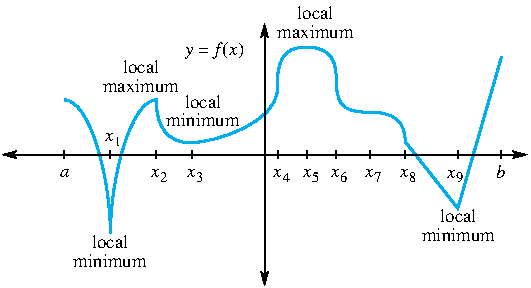
\includegraphics[width=20pc]{figsamp.pdf}
%
% when using dvips, use .eps file:
% 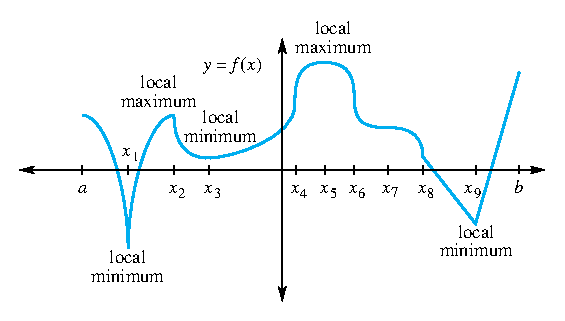
\includegraphics[width=20pc]{figsamp.eps}
%
% If you don't specify the file extension, 
% \includegraphics will insert the right file:
%\centerline{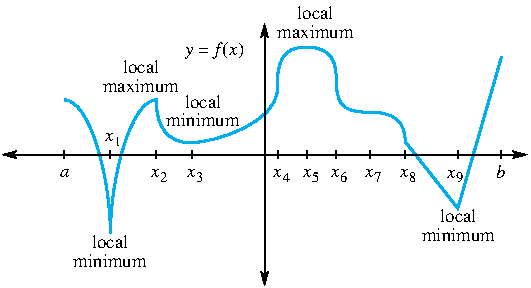
\includegraphics[height=1.5in]{figsamp}}
%\caption{Short caption}
%\label{figone}
%\end{figure}

%\begin{figure}[ht!]
%\centerline{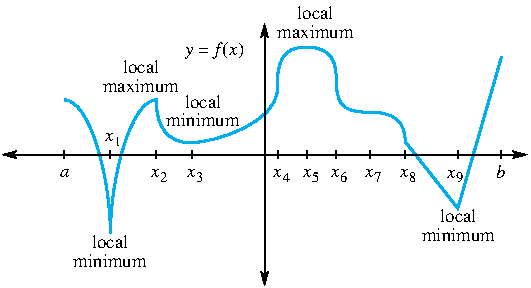
\includegraphics[angle=45,height=2in]{figsamp}}
%\caption{The figure caption should begin with an overall descriptive
%statement of the figure followed by additional text. They should be
%immediately after each figure.  Figure parts are indicated with
%lower-case letters ({\bf a, b, c}\ldots).  For initial submission, please place
%both the figures and captions in the text near where they are cited.}
%\label{fig:mean_and_slope}
%\end{figure}


%\begin{table}
%\caption{Start this caption with a short description of your
%table.
%Large tables
%especially presenting rich data should be presented as separate excel
%or .cvs files, not as part of the main text.}
%== Table Here ==
%\end{table}

%
% ---------------
% EXAMPLE TABLE
%
%\begin{table}
%\caption{Time of the Transition Between Phase 1 and Phase 2$^{a}$}
%\centering
%\begin{tabular}{l c}
%\hline
% Run  & Time (min)  \\
%\hline
%  $l1$  & 260   \\
%  $l2$  & 300   \\
%  $l3$  & 340   \\
%  $h1$  & 270   \\
%  $h2$  & 250   \\
%  $h3$  & 380   \\
%  $r1$  & 370   \\
%  $r2$  & 390   \\
%\hline
%\multicolumn{2}{l}{$^{a}$Table note text here.}
%\end{tabular}
%\end{table}


% See below for how to make sideways figures or tables.

% AGU prefers the use of {sidewaystable} over {landscapetable} as it causes fewer problems.
%
% \begin{sidewaysfigure}
% 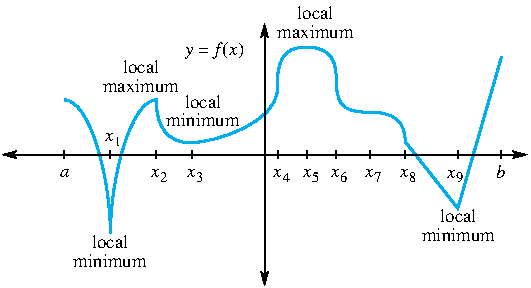
\includegraphics[width=20pc]{figsamp}
% \caption{Caption here}
% \label{newfig}
% \end{sidewaysfigure}
%
% \begin{sidewaystable}
% \caption{Caption here}
%\label{tab:signif_gap_clos}
% \begin{tabular}{ccc}
%one&two&three\\
%four&five&six
% \end{tabular}
% \end{sidewaystable}

%\clearpage

%% ------------------------------------------------------------------------ %%
%\section*{Citations}

% Please use ONLY \citet and \citep for reference citations.
% DO NOT use other cite commands (e.g., \cite, \citeyear, \nocite, \citealp, etc.).

%\subsection*{Cites made with \tt\string\citet\string{\string}}
%...as shown by \citet{Boug10}, \citet{Buiz07}, \citet{Fra10},
%\citet{Ghel00}, and \citet{Leit74}. 

%\subsection*{Cites made with \tt\string\citep\string{\string}}
%...as shown by \citep{Boug10}, \citep{Buiz07}, \citep{Fra10},
%\citep{Ghel00, Leit74}. 

%...has been shown \citep [e.g.,][]{Boug10,Buiz07,Fra10}.




%%% End of body of article

%%%%%%%%%%%%%%%%%%%%%%%%%%%%%%%%
%% Optional Appendix goes here
%
% \appendix resets counters and redefines section heads
% but doesn't print anything.
% After typing \appendix
%
%\section{Here Is Appendix Title}
% will show
% A: Here Is Appendix Title
%
%\appendix
%\section{Here is a sample appendix}
%This is an Appendix section.

%\subsection{subsection}
%This is an Appendix subsection.

%\subsubsection{subsubsection}
%This is an Appendix subsubsection.
%\begin{linenomath*}
%\begin{equation}asdf\end{equation}
%\end{linenomath*}

%%%%%%%%%%%%%%%%%%%%%%%%%%%%%%%%%%%%%%%%%%%%%%%%%%%%%%%%%%%%%%%%
%
% Optional Glossary, Notation or Acronym section goes here:
%
%%%%%%%%%%%%%%
% Glossary is only allowed in Reviews of Geophysics
%\begin{glossary}
%\term{Term}
% Term Definition here
%\term{Term}
% Term Definition here
%\term{Term}
% Term Definition here
%\end{glossary}

%
%%%%%%%%%%%%%%
% Acronyms
% \begin{acronyms}
% \acro{Acronym}
% Definition here
% \acro{EMOS}
% Ensemble model output statistics 
% \acro{ECMWF}
% Centre for Medium-Range Weather Forecasts
% \end{acronyms}

%
%%%%%%%%%%%%%%
% Notation 
% \begin{notation}
% \notation{$a+b$} Notation Definition here
% \notation{$e=mc^2$} 
% Equation in German-born physicist Albert Einstein's theory of special
%relativity that showed that the increased relativistic mass ($m$) of a
%body comes from the energy of motion of the body—that is, its kinetic
%energy ($E$)—divided by the speed of light squared ($c^2$).
% \end{notation}




%%%%%%%%%%%%%%%%%%%%%%%%%%%%%%%%%%%%%%%%%%%%%%%%%%%%%%%%%%%%%%%%
%
%  ACKNOWLEDGMENTS

\acknowledgments
This work benefits from support of VESPA/Europlanet.
The Europlanet 2020 Research Infrastructure is funded by the European Union
under the Horizon 2020 research and innovation program, grant agreement N.654208.


%%  REFERENCE LIST AND TEXT CITATIONS
%
% Either type in your references using
%
% \begin{thebibliography}{}
% \bibitem{}
% Text
% \end{thebibliography}
%
% Or, to use BibTeX:
%
% Follow these steps
%
% 1. Type in \bibliography{<name of your .bib file>} 
%    Run LaTeX on your LaTeX file.
%
% 2. Run BiBTeX on your LaTeX file.
%
% 3. Open the new .bbl file containing the reference list and
%   copy all the contents into your LaTeX file here.
%
% 4. Run LaTeX on your new file which will produce the citations.
%

\bibliography{epss_marmo}

% AGU does not want a .bib or a .bbl file. Please copy in the contents of your .bbl file here.


%\begin{thebibliography}{}


% % \bibitem[{\textit{Bell and Munoz}}(2008)]{Boug10} Bell, A.~H., and
% % Munoz, D.~P.  (2008). Activity in the superior colliculus reflects
% % dynamic interactions between voluntary and involuntary influences on
% % orienting behaviour. \textit{Eur. J. Neurosci.} 28, 1654--1660.

% % \bibitem[{\textit{Corbetta et~al.}}(1991)]{Buiz07} Corbetta, M.,
% % Miezin, F.~M., Dobmeyer, S., Shulman, G.~L., and Petersen, S.~E.
% % (1991). Selective and divided attention during visual discriminations
% % of shape, color, and speed: functional anatomy by positron emission
% % tomography. \textit{J.~Neurosci.} 11, 2383--2402.

% % \bibitem[{\textit{Borra et~al.}}(2014)]{Buiz98} Borra, E., Gerbella,
% % M., Rozzi, S., Tonelli, S., and Luppino, G.  (2014). Projections to
% % the superior colliculus from inferior parietal, ventral premotor, and
% % ventrolateral prefrontal areas involved in controlling goal-directed
% % hand actions in the macaque. \textit{Cereb. Cortex} 24, 1054--1065.

% % \bibitem[{\textit{Dorris et~al.}}(1997)]{Fra10}
% %  Dorris, M.~C.,
% % Par\'{e}, M., and Munoz, D.~P.  (1997). Neuronal activity in monkey
% % superior colliculus related to the initiation of saccadic eye
% % movements. \textit{J.~Neurosci.} 17, 8566--8579.

% % \bibitem[{\textit{Elsabbagh et~al.}}(2009)]{Ghel00} 
% % Elsabbagh, M.,
% % Volein, A., Holmboe, K., Tucker, L., Csibra, G., Baron-Cohen, S.,
% % et~al.  (2009). Visual orienting in the early broader autism
% % phenotype: disengagement. \textit{J.~Child Psychol. Psychiatry} 50,
% % 637--642.

% % \bibitem[{\textit{Fortin et~al.}}(1999)]{Gneit05} Fortin, S., Chabli,
% % A., Dumont, I., Shumikhina, S., Itaya, S.~K., and Molotchnikoff, S.
% % (1999). Maturation of visual receptive field properties in the rat
% % superior colliculus. \textit{bibain Res. Dev. Brain Res.} 1112,
% % 55--64.

% % \bibitem[{\textit{Felsen and Mainen}}(2008)]{Gneit07b} Felsen, G., and
% % Mainen, Z.~F.  (2008). Neural substrates of sensory-guided locomotor
% % decisions in the rat superior colliculus. \textit{Neuron} 60,
% % 137--148.

% % \bibitem[{\textit{Gattass and Desimone}}(1996)]{Haid14} Gattass, R.,
% % and Desimone, R.  (1996). Responses of cells in the superior
% % colliculus during performance of a spatial attention task in the
% % macaque. \textit{Rev. Bras. Biol.} 56, 257--279.

% % \bibitem[{\textit{Goldberg and Wurtz}}(1972)]{Hami00} Goldberg, M.~E.,
% % and Wurtz, R.~H.  (1972). Activity of superior colliculus in behaving
% % monkey. II. Effect of attention on neuronal responses.
% % \textit{J.~Neurophysiol.} 35, \hbox{560--574}.

% % \bibitem[{\textit{Krauzlis}}(2003)]{Kendall} Krauzlis, R.~J.  (2003).
% % Neuronal activity in the rostral superior colliculus related to the
% % initiation of pursuit and saccadic eye movements.
% % \textit{J.~Neurosci.} 23, 4333--4344.

% % \bibitem[{\textit{Heesy}}(2009)]{Leit74} 
% % Heesy, C.~P.  (2009). Seeing
% % in stereo: the ecology and evolution of primate binocular vision and
% % stereopsis. \textit{Evol. Anthropol.} 18, 21--35.

% % \bibitem[{\textit{Hilbig et~al.}}(2000)]{Mann45} Hilbig, H., Bidmon,
% % H.~J., Ettrich, P., and M\"{u}ller, A.  (2000). Projection neurons in
% % the superficial layers of the superior colliculus in the rat: a
% % topographic and quantitative morphometric analysis.
% % \textit{Neuroscience} 96, 109--119.

% % \bibitem[{\textit{Ignashchenkova et~al.}}(2004)]{Math76}
% % Ignashchenkova, A., Dicke, P.~W., Haarmeier, T., and Their, P.
% % (2004). Neuron-specific contribution of the superior colliculus to
% % overt and covert shifts of attention. \textit{Nat. Neurosci.} 7,
% % 56--64.

% \bibitem[{\textit{Krauzlis et~al.}}(2013)]{Palm00} Krauzlis, R.~J.,
% Lovejoy, L.~P., and Z\'{e}non, A.  (2013). Superior colliculus and
% visual spatial attention. \textit{Annu. Rev. Neurosci.} 36, 165--182.

% \bibitem[{\textit{Kustov and Robinson}}(1996)]{Papp09} Kustov, A.~A.,
% and Robinson, D.~L.  (1996). Shared neural control of attentional
% shifts and eye movements. \textit{Nature} 384, 74--77.

% \bibitem[{\textit{Landry and Bryson}}(2004)]{Park08} Landry, R., and
% Bryson, S.~E.  (2004). Impaired disengagement of attention in young
% children with autism. \textit{J.~Child Psychol. Psychiatry} 45,
% 1115--1122.

% \bibitem[{\textit{Kobayashi et~al.}}(2003)]{R2013} Kobayashi, T.,
% Tran, A.~H., Nishijo, H., Ono, T., and Matsumoto, G.  (2003).
% Contribution of hippocampal place cell activity to learning and
% formation of goal-directed navigation in rats. \textit{Neuroscience}
% 117, 1025--1035.

% \bibitem[{\textit{McHaffie et~al.}}(2005)]{Raft05} McHaffie, J.~G.,
% Stanford, T.~R., Stein, B.~E., Coizet, V., and Redgrave, P.  (2005).
% Subcortical loops through the basal ganglia. \textit{Trends Neurosci.}
% 28, 401--407.

% \bibitem[{\textit{McPeek and Keller}}(2004)]{Rich13} McPeek, R.~M.,
% and Keller, E.~L.  (2004). Deficits in saccade target selection after
% inactivation of superior colliculus. \textit{Nat. Neurosci.} 7,
% 757--763.

% \bibitem[{\textit{M\"{u}ller et~al.}}(2005)]{Scheu14} M\"{u}ller,
% J.~R., Philiastides, M.~G., and Newsome, W.~T.  (2005).
% Microstimulation of the superior colliculus focuses attention without
% moving the eyes. \textit{Proc. Natl. Acad. Sci. U.S.A.} 102, 524--529.

% \bibitem[{\textit{Munoz and Istvan}}(1998)]{ScheueBue13} Munoz, D.~P.,
% and Istvan, P.~J.  (1998). Lateral inhibitory interactions in
% the intermediate layers of the monkey superior colliculus.
% \textit{J.~Neurophysiol.} 79, 1193--1209.

%\end{thebibliography}

%%%%%%%%%%%%%%%%%%%%%%%%%%%%%%%%%%%%%%%%%
% Track Changes:
% To add words, \added{<word added>}
% To delete words, \deleted{<word deleted>}
% To replace words, \replace{<word to be replaced>}{<replacement word>}

% At the end of the document, use \listofchanges, which will list the
% changes and the page and line number where the change was made.

% When final version, \listofchanges will not produce anything,
% \added{} word will be printed, \deleted{} will take away the word,
% \replaced{}{} will print only the 2nd argument.

%%%
\listofchanges
%%%

\end{document}

%%%%%%%%%%%%%%%%%%%%%%%%%%%%%%%%%%%%%
%% Supporting Information
%% (Optional) See AGUSuppInfoSamp.tex/pdf for requirements 
%% for Supporting Information.
%%%%%%%%%%%%%%%%%%%%%%%%%%%%%%%%%%%%%


%%%%%%%%%%%%%%%%%%%%%%%%%%%%%%%%%%%%%%%%%%%%%%%%%%%%%%%%%%%%%%%

More Information and Advice:

%% ------------------------------------------------------------------------ %%
%
%  SECTION HEADS
%
%% ------------------------------------------------------------------------ %%

% Capitalize the first letter of each word (except for
% prepositions, conjunctions, and articles that are
% three or fewer letters).

% AGU follows standard outline style; therefore, there cannot be a section 1 without
% a section 2, or a section 2.3.1 without a section 2.3.2.
% Please make sure your section numbers are balanced.
% ---------------
% Level 1 head
%
% Use the \section{} command to identify level 1 heads;
% type the appropriate head wording between the curly
% brackets, as shown below.
%
%An example:
%\section{Level 1 Head: Introduction}
%
% ---------------
% Level 2 head
%
% Use the \subsection{} command to identify level 2 heads.
%An example:
%\subsection{Level 2 Head}
%
% ---------------
% Level 3 head
%
% Use the \subsubsection{} command to identify level 3 heads
%An example:
%\subsubsection{Level 3 Head}
%
%---------------
% Level 4 head
%
% Use the \subsubsubsection{} command to identify level 3 heads
% An example:
%\subsubsubsection{Level 4 Head} An example.
%
%% ------------------------------------------------------------------------ %%
%
%  IN-TEXT LISTS
%
%% ------------------------------------------------------------------------ %%
%
% Do not use bulleted lists; enumerated lists are okay.
% \begin{enumerate}
% \item
% \item
% \item
% \end{enumerate}
%
%% ------------------------------------------------------------------------ %%
%
%  EQUATIONS
%
%% ------------------------------------------------------------------------ %%

% Single-line equations are centered.
% Equation arrays will appear left-aligned.

Math coded inside display math mode \[ ...\]
 will not be numbered, e.g.,:
 \[ x^2=y^2 + z^2\]

 Math coded inside \begin{equation} and \end{equation} will
 be automatically numbered, e.g.,:
 \begin{equation}
 x^2=y^2 + z^2
 \end{equation}


% To create multiline equations, use the
% \begin{eqnarray} and \end{eqnarray} environment
% as demonstrated below.
\begin{eqnarray}
  x_{1} & = & (x - x_{0}) \cos \Theta \nonumber \\
        && + (y - y_{0}) \sin \Theta  \nonumber \\
  y_{1} & = & -(x - x_{0}) \sin \Theta \nonumber \\
        && + (y - y_{0}) \cos \Theta.
\end{eqnarray}

%If you don't want an equation number, use the star form:
%\begin{eqnarray*}...\end{eqnarray*}

% Break each line at a sign of operation
% (+, -, etc.) if possible, with the sign of operation
% on the new line.

% Indent second and subsequent lines to align with
% the first character following the equal sign on the
% first line.

% Use an \hspace{} command to insert horizontal space
% into your equation if necessary. Place an appropriate
% unit of measure between the curly braces, e.g.
% \hspace{1in}; you may have to experiment to achieve
% the correct amount of space.


%% ------------------------------------------------------------------------ %%
%
%  EQUATION NUMBERING: COUNTER
%
%% ------------------------------------------------------------------------ %%

% You may change equation numbering by resetting
% the equation counter or by explicitly numbering
% an equation.

% To explicitly number an equation, type \eqnum{}
% (with the desired number between the brackets)
% after the \begin{equation} or \begin{eqnarray}
% command.  The \eqnum{} command will affect only
% the equation it appears with; LaTeX will number
% any equations appearing later in the manuscript
% according to the equation counter.
%

% If you have a multiline equation that needs only
% one equation number, use a \nonumber command in
% front of the double backslashes (\\) as shown in
% the multiline equation above.

% If you are using line numbers, remember to surround
% equations with \begin{linenomath*}...\end{linenomath*}

%  To add line numbers to lines in equations:
%  \begin{linenomath*}
%  \begin{equation}
%  \end{equation}
%  \end{linenomath*}
